\section{Mémoire unifiée}
\begin{frame}[fragile]
    \frametitle{Accès mémoire unifié}
\begin{block}{Un même pointeur CPU/GPU}
    \begin{itemize}
        \item<+-> La mémoire unifiée est allouée grâce à la fonction \texttt{cudaMallocManaged}.
        \item<+-> Elle est libérée en appelant \texttt{cudaFree}
        \item<+-> Le pointeur obtenu est utilisable sur l'hôte \textbf{et} sur le GPU.
        \item<+-> Cela permet d'éliminer la plupart du temps les appels à \texttt{cudaMemcpy}.
        \item<+-> Le décorateur \texttt{\_\_managed\_\_} peut également être utilisé devant un nom de variable globale.
    \end{itemize}
\end{block}
\end{frame}
\begin{frame}
    \frametitle{Mémoire unifiée}
\begin{block}{Noyau}
   \begin{tabular}{cc}
        \begin{minipage}{0.45\textwidth}
 \begin{figure}[htbp]
    \centering
   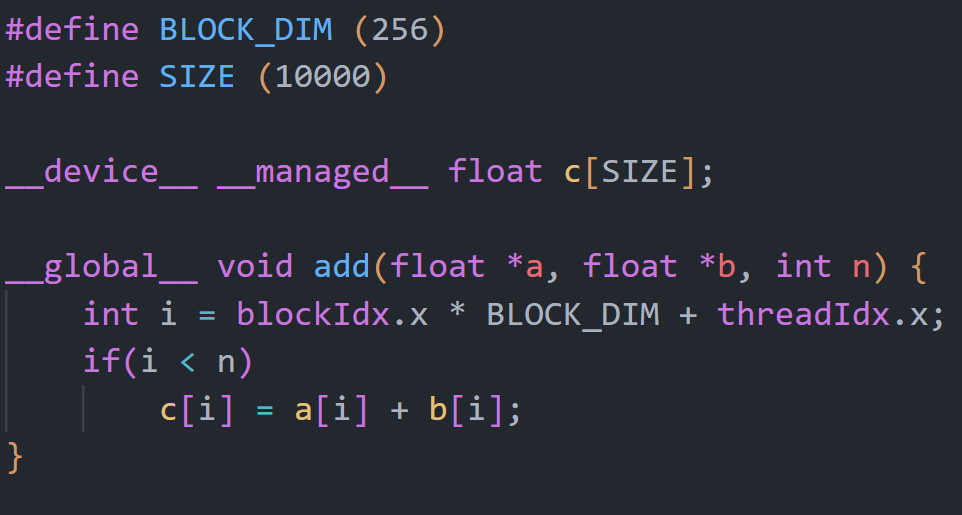
\includegraphics[width=\textwidth]{managed_kernel.png}
    \caption{Utilisation de la mémoire unifiée.}
    \label{fig:Noyau}
\end{figure}
        \end{minipage} & 
        \begin{minipage}{0.45\textwidth}
            \begin{itemize}
                \item<+-> On notera la déclaration de la variable globale de retour.
           \end{itemize}
        \end{minipage}
\end{tabular}
\end{block}
\end{frame}
\begin{frame}[fragile]
    \frametitle{Mémoire unifiée}
\begin{block}{Programme principal}
   \begin{tabular}{cc}
        \begin{minipage}{0.45\textwidth}
 \begin{figure}[htbp]
    \centering
   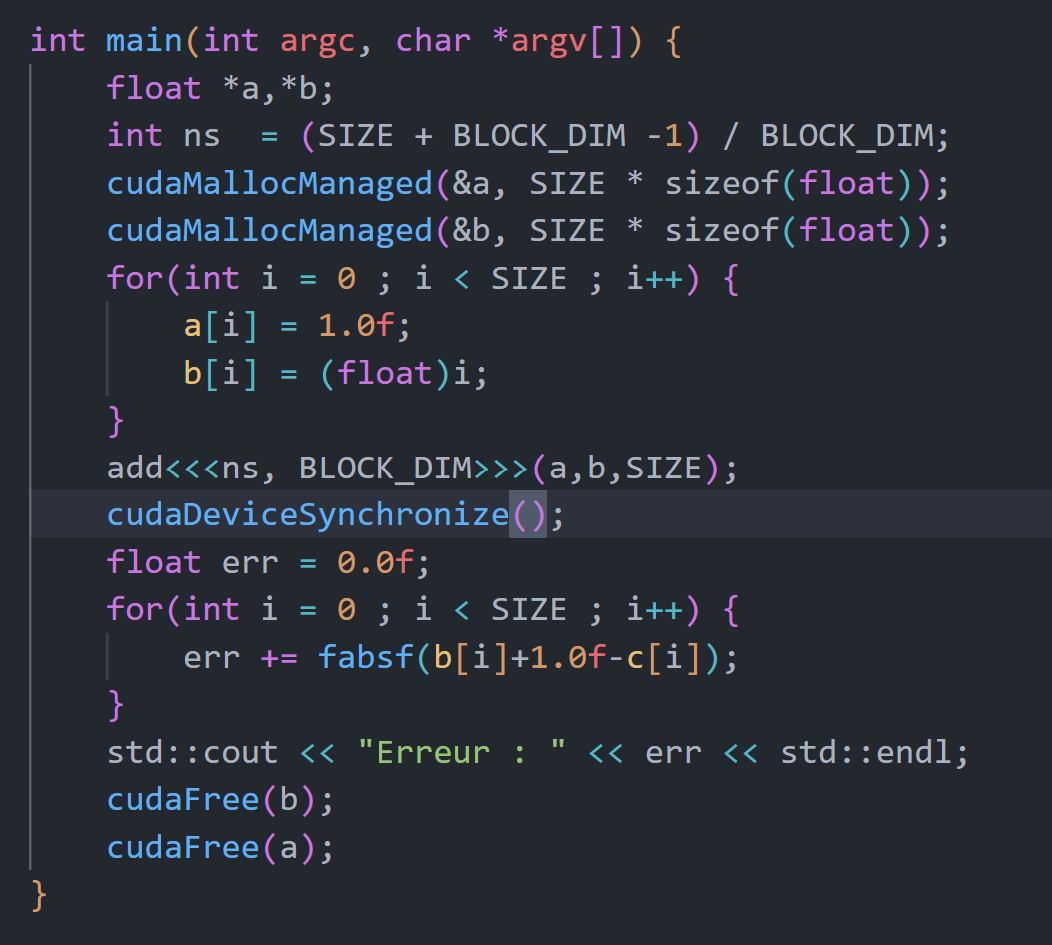
\includegraphics[width=\textwidth]{managed_launch.png}
    \caption{Allocation sur CPU.}
    \label{fig:managed_launch}
\end{figure}
        \end{minipage} & 
        \begin{minipage}{0.45\textwidth}
            \begin{itemize}
                \item<+-> L'utilisation de la mémoire unifiée permet de se dispenser d'opérations de copie.
                \item<+-> Le décorateur \texttt{\_\_managed\_\_} déclare la variable sur le CPU et le GPU.
           \end{itemize}
        \end{minipage}
\end{tabular}
\end{block}
\end{frame}